\documentclass[../TST.tex]{subfiles}
\begin{document}
\begin{pproblem}
A convex lens of diameter $D=\qty{10}{cm}$ and focal length $f=\qty{1}{m}$ is cut into two identical halves, removing a glass layer of thickness $a=\qty{0.5}{mm}$. The two halves are then stuck back together. A point source of monochromatic light of wavelength $\lambda=\qty{500}{nm}$ is placed in the focal plane of the system. A screen is placed perpendicularly to the optical axis at a distance of $L=\qty{10}{m}$ on the other side of the lens.
\end{pproblem}
\begin{subpart}
\item Find the distance $\Delta x$ between the maxima of the resulting interference pattern.
\item Find the number of maxima on the screen $N$.
\item Approximately at what size of the point source $\delta$ does the interference pattern vanish?
\item Find the distance $L_\mathrm{max}$ at which the screen should be placed so that the number of maxima is largest. What is this number $N_\mathrm{max}$?\\
\end{subpart}

\ifprob \else
\begin{solution}
(a) Each of two halves acts exactly like the lens it came from, in that any ray refracted through that half doesn't know the other half is now missing. After we stick the two halves back together, it's as if we have two identical lenses with centres at $y=-a/2$ and $y=+a/2$. The source is now off-axis for both of them, so the rays passing through the two halves will diverge in different directions. These directions are given by the two lines that connect the source to the centres. The angle these make with the optical axis is $\theta = \frac{a}{2f}$.  The parallel beams from the two halves of the lens will overlap, resulting in interference:\\
\begin{center}
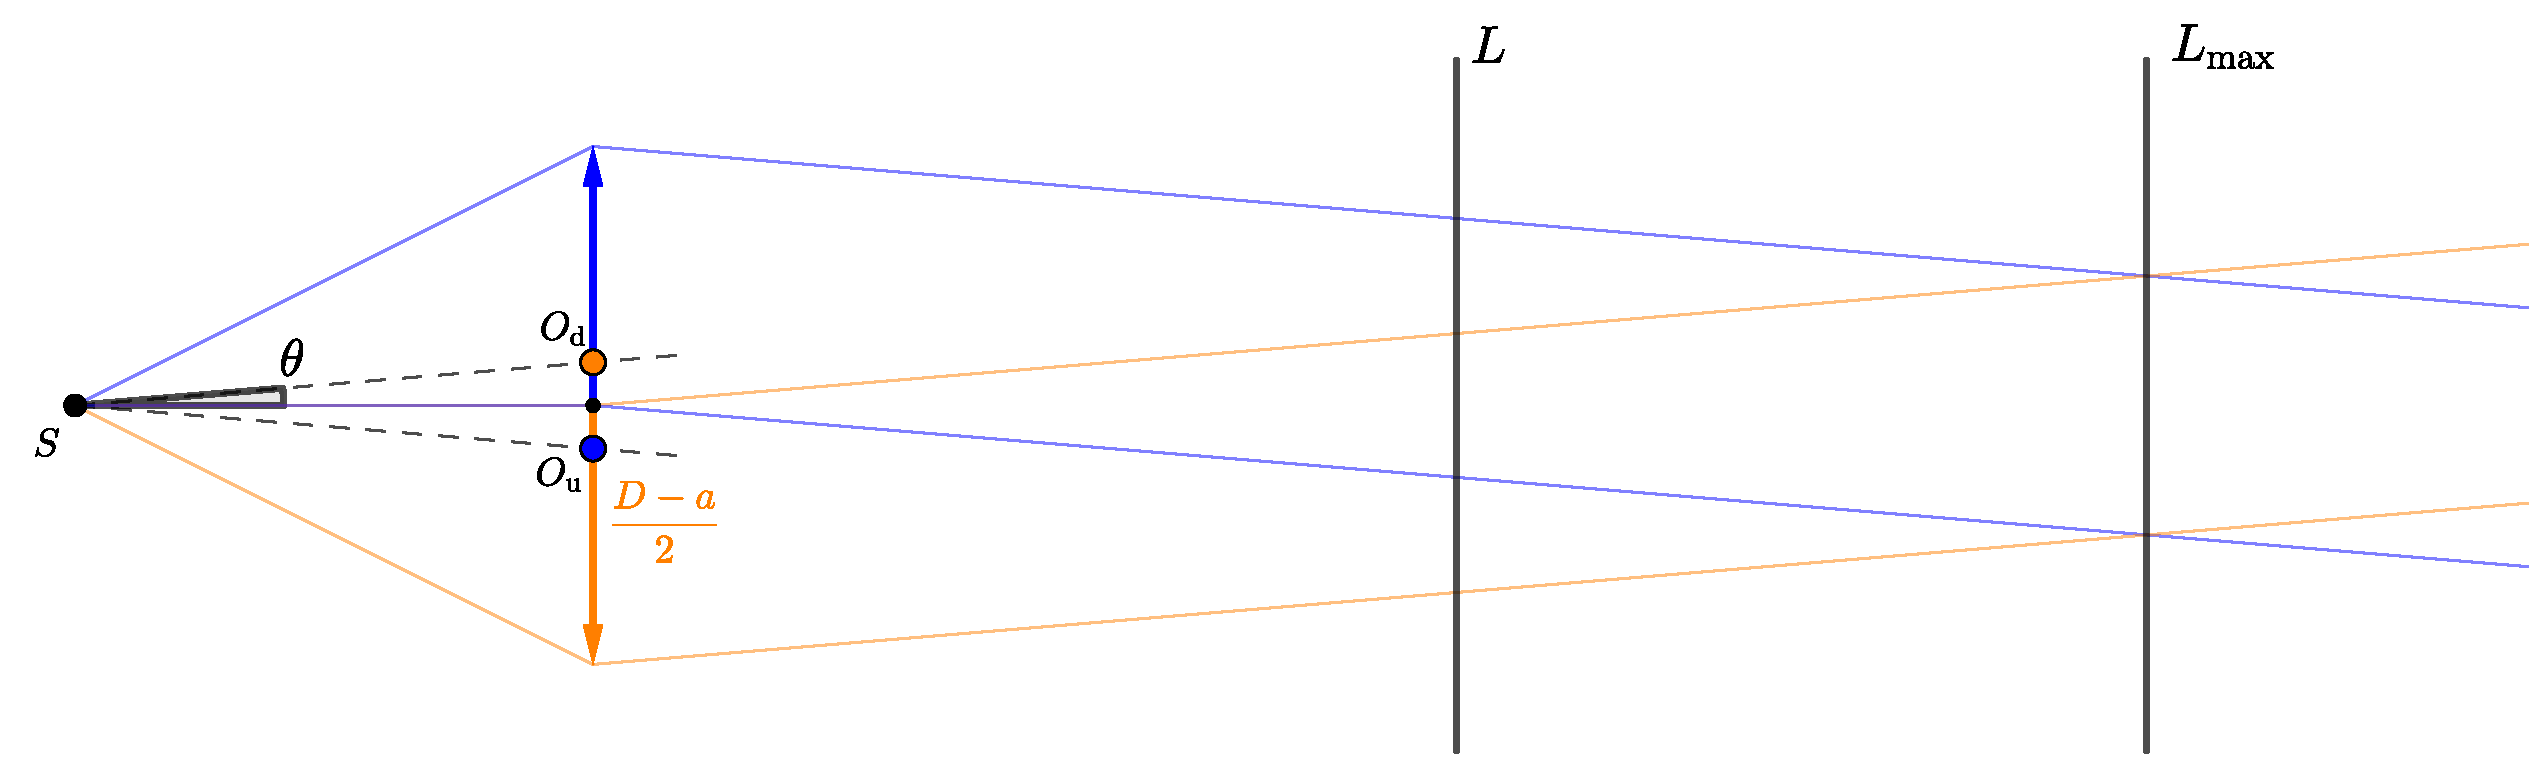
\includegraphics[width=0.9\textwidth]{fig/a2009_s61.pdf}
\end{center}

Let us find the distance between the maxima on the screen, given that the angle between the beams is $2\theta$. Consider some maximum at point $A$. At that point on the screen, the two interfering waves have a phase difference of $2\pi k$, $k\in \mathbb{Z}$. As we move downwards along the screen (towards the next maximum $B$), the phases of the waves when they touch the screen will vary. The rays coming from the top will strike the screen with a greater phase, while those coming from the bottom will strike it with a lesser phase. Eventually, at the next maximum $B$, the phase of the rays coming from the top will have increased by $\pi$, while the phase of those from the bottom will have gone down by $\pi$, for a total extra phase difference of $2\pi$. 
\begin{center}
	\hspace{1cm}
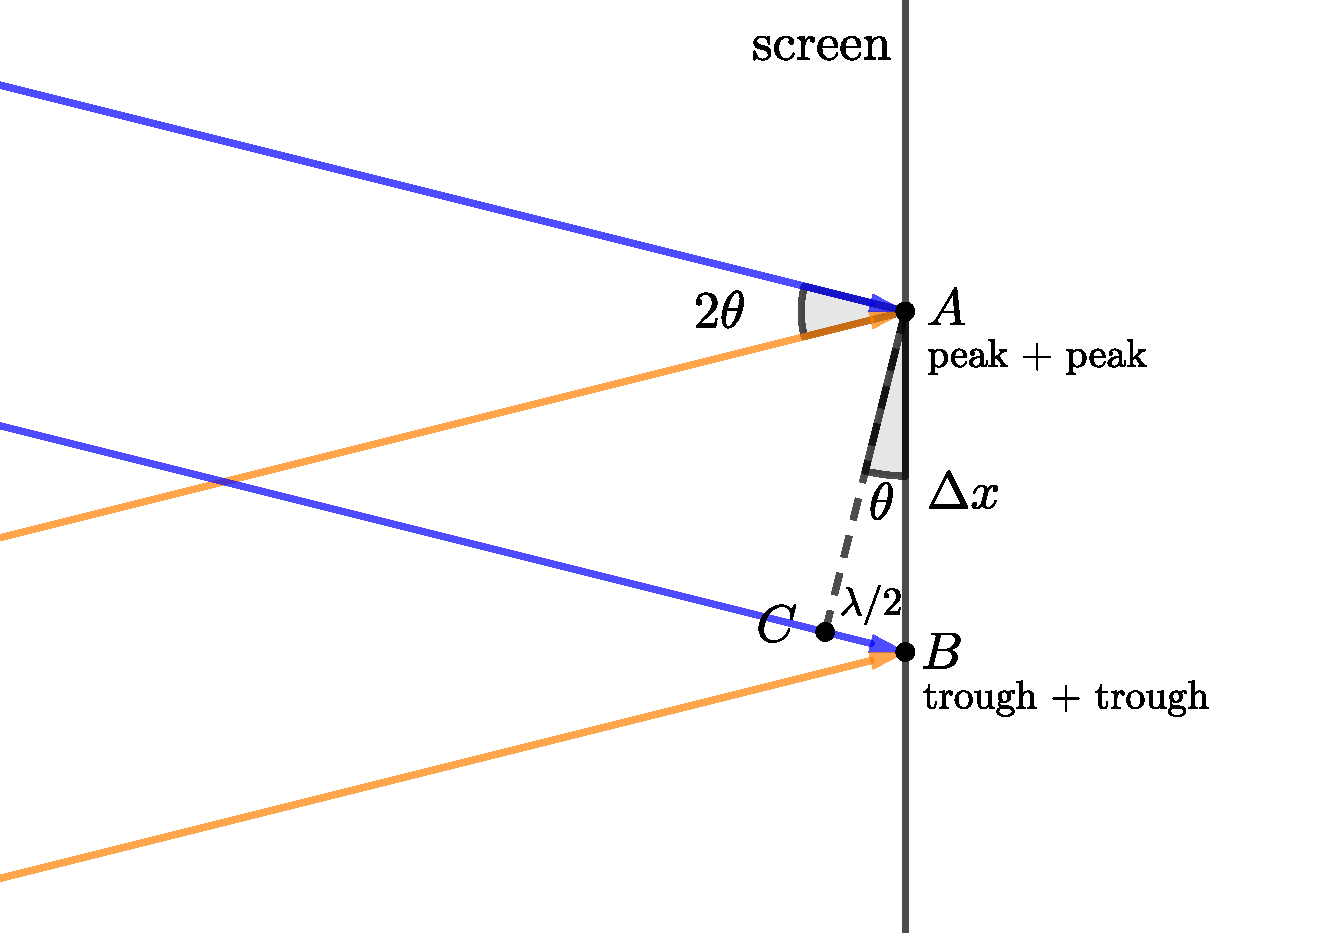
\includegraphics[width=0.5\textwidth]{fig/a2009_s62.pdf}
\end{center}

We then deduce that the segment $BC$ has to correspond to a phase difference of $\pi$, meaning that its length is $\lambda/2$. Since $\theta$ is small, we can write $\theta=\frac{\lambda/2}{\Delta x}$. This yields 
\begin{equation*}
	\boxed{\Delta x = \frac{\lambda f}{a}=\qty{1}{mm}.}
\end{equation*}
Note that it doesn't matter how far the screen is.\\

(b) We first need to find the dimensions of the zone where the rays can interfere. This zone is a parallelogram with orthogonal diagonals, meaning it is a rhombus with an angle of $2\theta$. Also, we see that its maximum width is $\frac{D-a}{2}$, which is the size of each of the halves. This width is reached at some distance $L_\mathrm{max}$ from the lens which satisfies $(2\theta)L_\mathrm{max}=\frac{D-a}{2}$. Then $L_\mathrm{max}\approx \frac{(D-a)f}{2a}=\qty{99.5}{m}$. In this part of the problem, the distance to the screen is much less, $L=\qty{10}{m}$. The width of the interference zone at that distance is 
\begin{equation*}
w=(2\theta)L=\frac{aL}{f}=\qty{5}{mm}
.
\end{equation*}
This isn't that much compared to $\Delta x$, so we need to check explicitly how all the maxima fit within this zone. By symmetry, there will be a maximum at the centre of the screen where the optical axis is. Now we arrange maxima in steps of $\Delta x$ around the central maximum. We have $\frac{w}{2}=\qty{2.5}{mm}$ of available space on each side for that. We can only go up to $2\Delta x =\qty{2}{mm}$ on each side. This is a total of $1+2\cdot 2 = 5$ maxima. The general form of the answer is
\begin{equation*}
	N=1+2\left\lfloor \frac{w/2}{\Delta x}\right\rfloor = \boxed{1+2\left\lfloor \left(\frac{a}{f}\right)^2 \frac{L}{2\lambda}  \right\rfloor = 5.}
\end{equation*}
(c) Assume the source is a sphere of diameter $\delta$. Each individual surface element of the sphere can be treated as a separate point source with its own interference pattern. The surface elements have different positions on the $y$-axis, which means their interference patterns are offset from each other ($x$-axis displacements won't matter to first order). In order to find the offset, we will consider two surface elements $S_1$ and $S_2$, one at $y=0$ and the other at $y=d\leq \delta$. Let us see what happens at some fixed point on the screen $D$. To simplify the calculations, we will work with a point at $x=L$ and $y=0$. Each source emits a pair of rays that end up at $D$ after passing through the top and bottom half of the lens, respectively. We now need to construct these rays on a diagram. The sources are in the focal plane, meaning that all refracted rays travel in the same direction as the lines connecting the source to the centre of each half. We draw these lines ($S_1O_\mathrm{d}$, $S_1O_\mathrm{u}$, $S_2O_\mathrm{d}$, $S_2O_\mathrm{u}$), and work back from $D$ to construct rays parallel to them.
\begin{center}
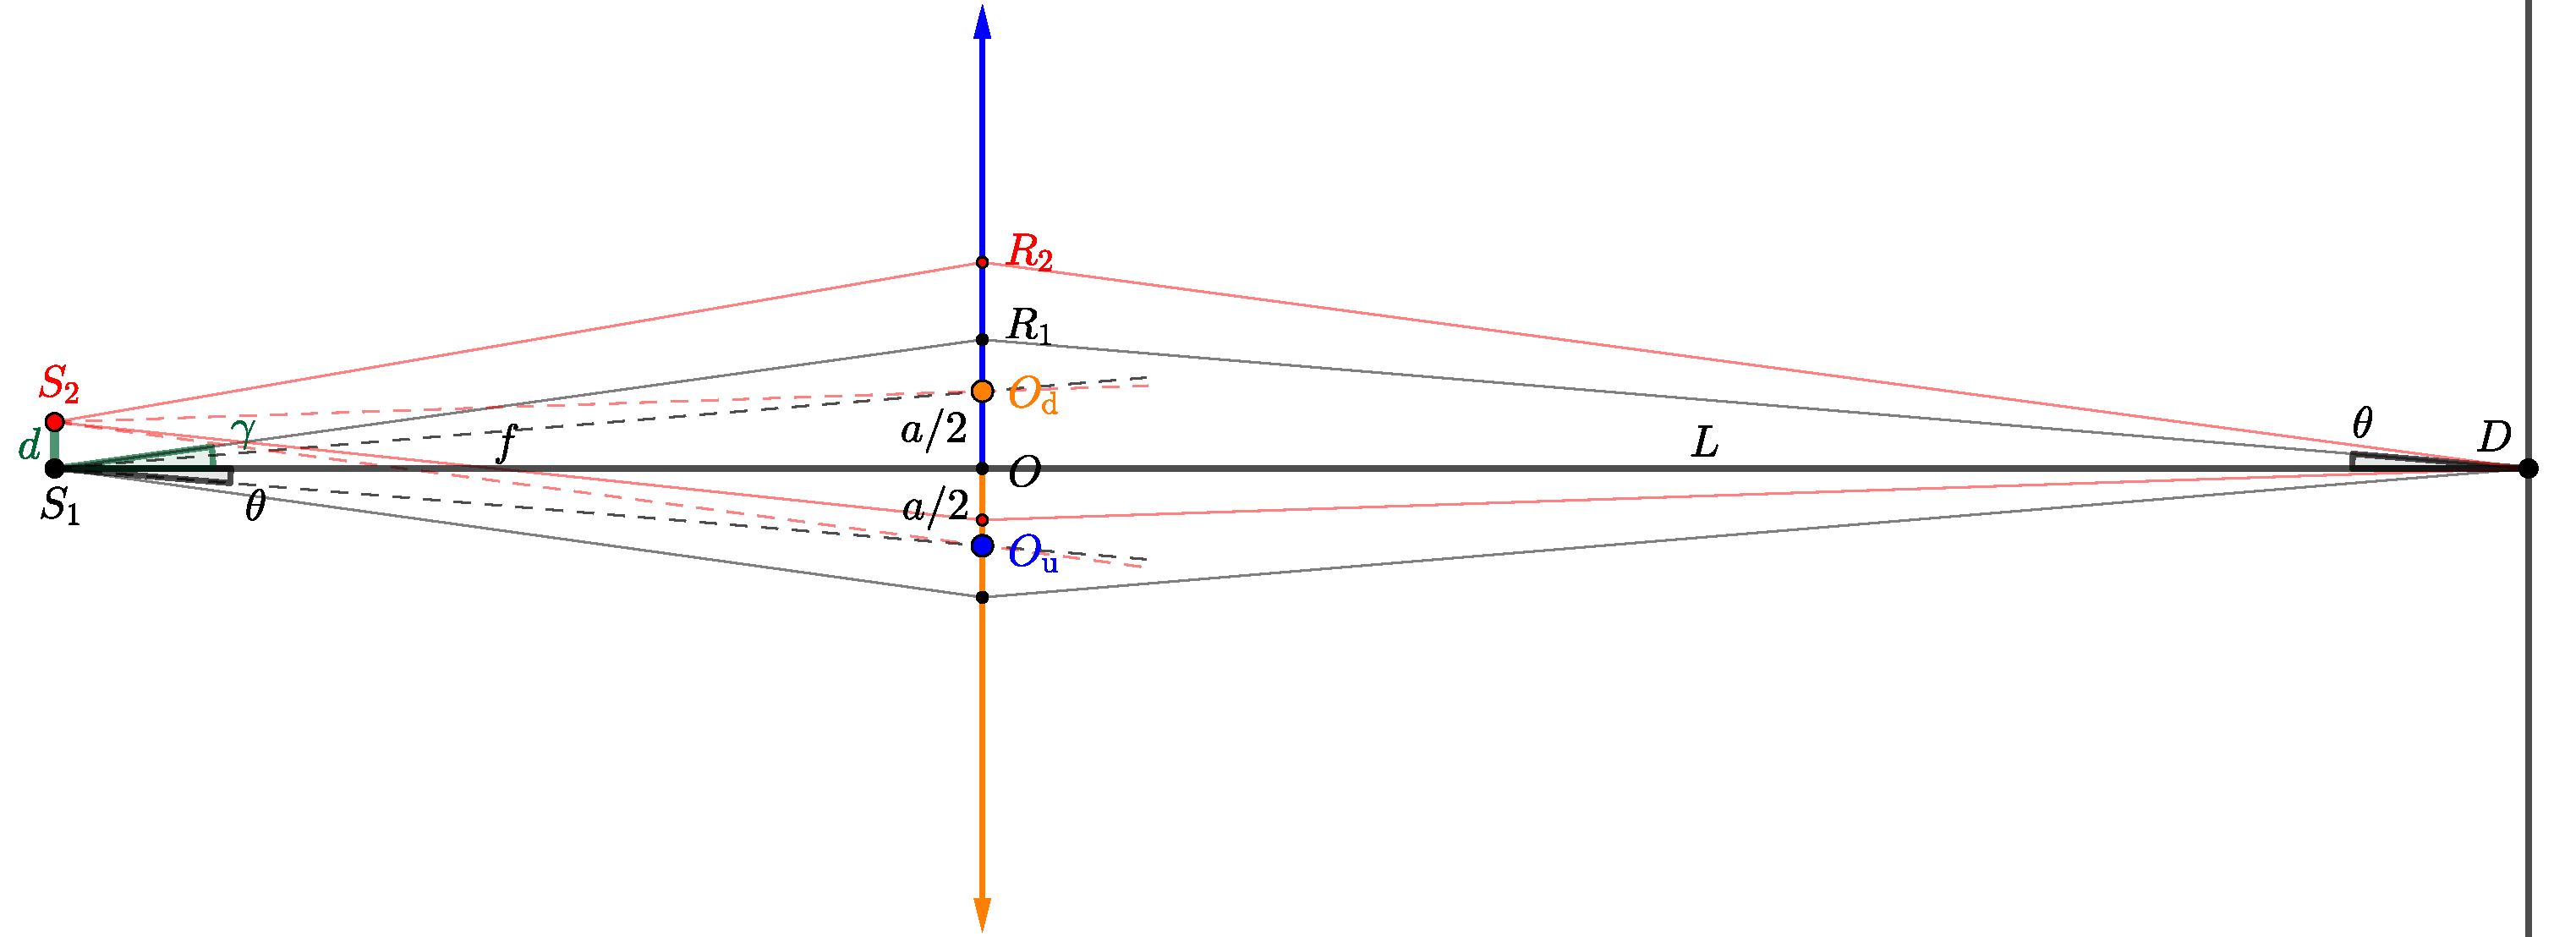
\includegraphics[width=1\textwidth]{fig/a2009_s63.pdf}
\end{center}

Due to symmetry, the rays coming from $S_1$ terminate at $D$ in phase. However, the two rays from $S_2$ will carry some phase difference. To find it, we first compare the phase difference of rays $S_1R_1D$ and $S_2R_2D$. Here you need to consider the path difference both in the air and within the lens. This is hard to do by hand, but there's a trick. The reversed rays $DR_1S_1$ and $DR_2S_2$ both seem to emanate from point $D$, and they will eventually converge at the image of $D$ from the top half (say, $D'$, not shown in the figure). From Fermat's principle of equal travel time, we know that these rays will arrive at $D'$ with no phase difference. Therefore, the phase difference of our two rays is equal to that of the two segments $D'S_2$ and $D'S_1$. But this is a standard configuration with a path difference of $d\sin{\gamma}$, or a phase difference of $\frac{2\pi}{\lambda}d\sin{\gamma}$. Repeating this procedure for the second ray from $S_2$, we find the same phase difference with respect to the ray from $S_1$ passing through the bottom half, albeit with the opposite sign. We conclude that the two rays from $S_2$ interfere with a phase difference of $\frac{4\pi}{\lambda}d\sin{\gamma}\approx\frac{4\pi}{\lambda}d{\gamma}$.\\[5pt]
To obtain $\gamma$, note that $\angle ODR_1=\angle O_\mathrm{u}S_1O=\theta$, and then write $OR_1=\gamma f=\theta L$. Thus, the rays from $S_2$ have a phase difference of 
\begin{equation*}
\Delta\phi=\frac{2\pi aLd}{\lambda f^2}
.
\end{equation*}
An object of size $\delta$ should then supply a range of phase differences between $0$ and $\frac{2\pi aL\delta}{\lambda f^2}$ at $D$. This smears out the minima and the maxima. For example, at the point where rays used to interfere at a phase difference $\phi$ (back when we had a point source $S$), we now have a distribution of phase differences $\left[\phi-\frac{\pi a L \delta}{\lambda f^2},\,\phi+\frac{\pi a L \delta }{\lambda f^2} \right]$ centered at $\phi$. For the interference pattern to vanish, the maxima should be indistinguishable from the minima. To check this, we will use something akin to the Rayleigh criterion. We will assume that a minimum and a maximum become indistinguishable when the tail of the distribution for the minimum lies at the centre of the distribution for the maximum:\\

\begin{center}
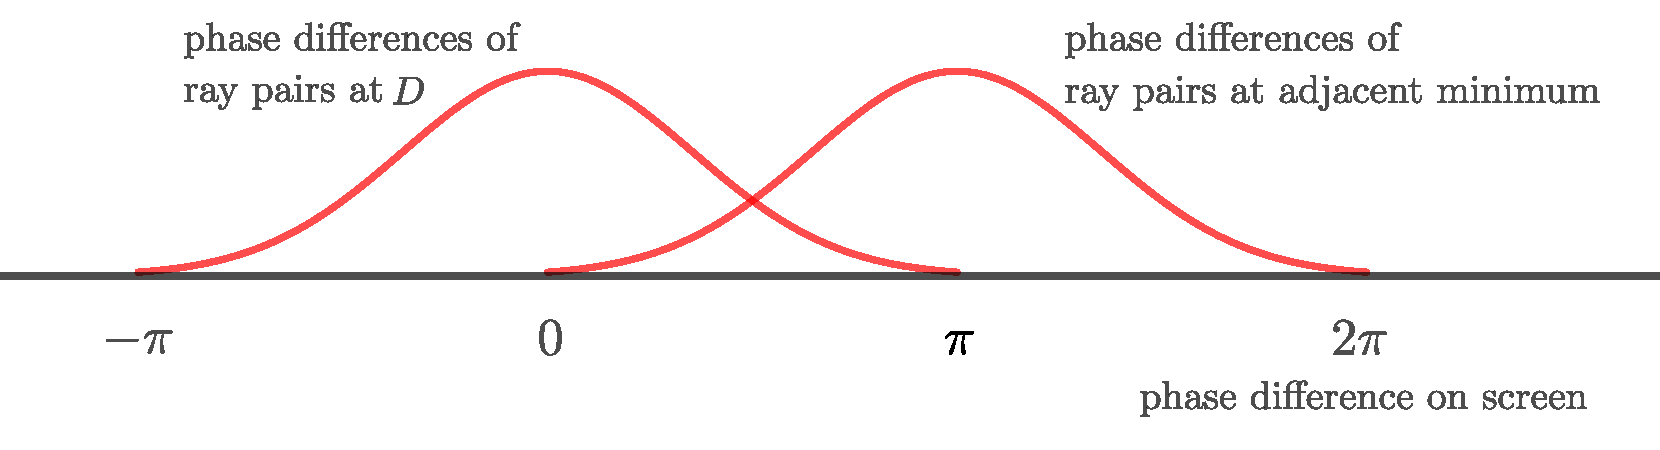
\includegraphics[width=0.8\textwidth]{fig/a2009_s64.pdf}
\end{center}

In that case, $\frac{\pi a L\delta}{\lambda f^2}=\pi$, or 
\begin{equation*}
	\boxed{\delta = \frac{\lambda f^2}{aL} = \qty{0.1}{mm}.}
\end{equation*}
This answer seems to make sense -- as we increase $L$, phase differences accumulate more easily, so the setup fails at a lesser $\delta$. However, I'd still like someone to \underline{confirm} it, because I couldn't find anything similar in the literature. Please email me if you have read my solution and you are confident that it is correct. \\

(d) The distance between adjacent maxima is always $\Delta x$, so the number of maxima is largest when the zone of interference is at its widest. As we found previously, this corresponds to a distance of 
\begin{equation*}
	\boxed{L_\mathrm{max}=\frac{(D-a)f}{2a}=\qty{99.5}{m}.}
\end{equation*}
The width of the zone at that point is $\frac{D-a}{2}$. We reuse the general formula for the number of maxima to find
\begin{equation*}
\boxed{N_\mathrm{max}=1+2\left\lfloor \frac{(D-a)a}{2\lambda f}  \right\rfloor = 99.}
\end{equation*}
If we had approximated $(D-a)$ to $D$ too early, we would have instead got $N_\mathrm{max}=101$.
\end{solution}
\fi

\end{document}
